%------------------------------------------------------------------------------------------------------------------------
\chapter{次世代ピクセル検出器の量産}
\label{sec:singatapixel-devel}
%------------------------------------------------------------------------------------------------------------------------
%現行のにおける測定と同時に、
HL-LHCアップグレードに向けた内部飛跡検出器の総入れ替えのため、次世代ピクセル検出器の開発が進められている。現在、ITkに搭載するピクセル検出器量産の各組み立て工程における試験やそのシステム確立のため、試作器を用いたデモンストレーションが行われている。

日本では新型器量産の際に約$2000$個のモジュールを生産する予定である。次世代ピクセル検出器の量産の際に、効率の良い量産と統合されたピクセル検出器選定を行うため、品質試験結果を統合管理するシステムの開発が必要となる。


%------------------------------------------------------------------------------------------------------------------------
\section{次世代ピクセル検出器の組み立て部品}
\label{sec:component}
%------------------------------------------------------------------------------------------------------------------------
量産工程は、各組み立て機関に届いたセンサーとASICから作られるベアモジュールとフレキシブル基板の接着から始まる。本節では各部品の詳細について説明する。


%------------------------------------------------------------------------------------------------------------------------
\subsection{ベアモジュール}
\label{sec:bare}
%------------------------------------------------------------------------------------------------------------------------

ベアモジュールはセンサーとASICをバンプ接合することにより作られる。クアッドモジュールではセンサー1枚に対してASIC1枚、トリプレットモジュールではセンサー1枚に対してASIC1枚から構成される。ベアモジュールは通過する粒子を検出する。センサーを通過した荷電粒子は電子・ホール対を生成し、それにより得られる信号をASICを用いて増幅・整形を行う。\fref{fig:bare}にベアモジュールの全体図を示す。
\begin{figure}[tbp]
  \centering
  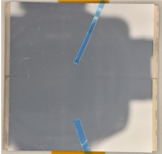
\includegraphics[height=5cm,keepaspectratio]{bare.png}
  \caption[ベアモジュール]{ベアモジュールの全体図。センサー側から見たものであり、左右にASICがはみ出している。これはフレキシブル基板につながるワイヤーのためのパッド部分である。}
  \label{fig:bare}
\end{figure}

%現在行われている試作器の組み立てではRD53AというASICを用いている。


%------------------------------------------------------------------------------------------------------------------------
\subsection{フレキシブル基板}
\label{sec:flex}
%------------------------------------------------------------------------------------------------------------------------

フレキシブル基板はセンサーの裏側(\fref{fig:bare}の上面)に接着、およびワイヤー配線によりASICと電気的に接続される。フレキシブル基板の全体図を\fref{fig:flex}に示す。フレキシブル基板は、以下の3つの役割を持つ。

\begin{figure}[tbp]
  \centering
  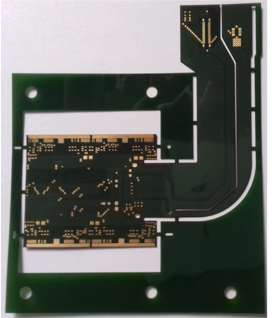
\includegraphics[height=6cm,keepaspectratio]{flex.png}
  \caption[フレックス基板]{フレックス基板の全体図\ \cite{itk}。}
  \label{fig:flex}
\end{figure}

フレキシブル基板は、以下の3つの役割を持つ。
\begin{itemize}
  \item ASICからの信号輸送  \\
  センサーから得られた信号はASICで増幅・整形され、フレキシブル基板に送られてくる。フレキシブル基板は送られてきた信号を後段のPCへ送る。
  \item 電源の供給 \\
  外部からの電源を、センサーとASICに供給する。センサーには、空乏領域を増加させるために$100\ \si{V}$程度のHV(\textbf{H}igh \textbf{V}oltage)をかける。ASICには、電源供給のために$5.6\ \si{V}$程度のLV(\textbf{L}ow \textbf{V}oltage)
  \item モジュールの制御システム(DCS: \textbf{D}etector \textbf{C}ontrol \textbf{S}ystem) \\
  モジュールの温度測定のために2つのNTC(\textbf{N}egative \textbf{T}emperature \textbf{C}oefficient)が配置されている。
\end{itemize}

%------------------------------------------------------------------------------------------------------------------------
\subsection{モジュールキャリア}
\label{sec:carrier}
%------------------------------------------------------------------------------------------------------------------------

モジュールキャリアはモジュールの運搬の際や品質試験を行う際に、モジュールを保護用の容器である。組み立てられたモジュールはASICとフレックス基板を繋ぐワイヤー部やセンサーの部分等が剥き出しになっているため、そのままの状態で品質試験を行うのはモジュール破損のリスクを伴う。モジュールキャリアでモジュールを保護することにより、安全に品質試験を行うことができる。

また、モジュールキャリアの別の役割として、モジュール周囲の湿度環境を一定に保つことが挙げられる。運転時に想定される最低温度は$-45\ \si{\degreeCelsius}$のため、品質管理試験ではペルチェ素子を用いた温度制御装置\footnote{KEKにおける次世代ピクセル検出器の量産では、東工大を中心に開発している温度制御システムを用いる。}を用いて最低$-45\ [\si{\degreeCelsius}]$までモジュールの周囲温度を下げる。その際、ピクセル検出器に結露が発生すると損傷のリスクを伴う。そのため、キャリア内に乾燥窒素ガスを流し込むことで氷点下におけるピクセル検出器への結露を防いでいる。

%------------------------------------------------------------------------------------------------------------------------
\section{次世代ピクセル検出器の組み立て工程}
\label{sec:assemble}
%------------------------------------------------------------------------------------------------------------------------
\begin{figure}[tbp]
  \centering
  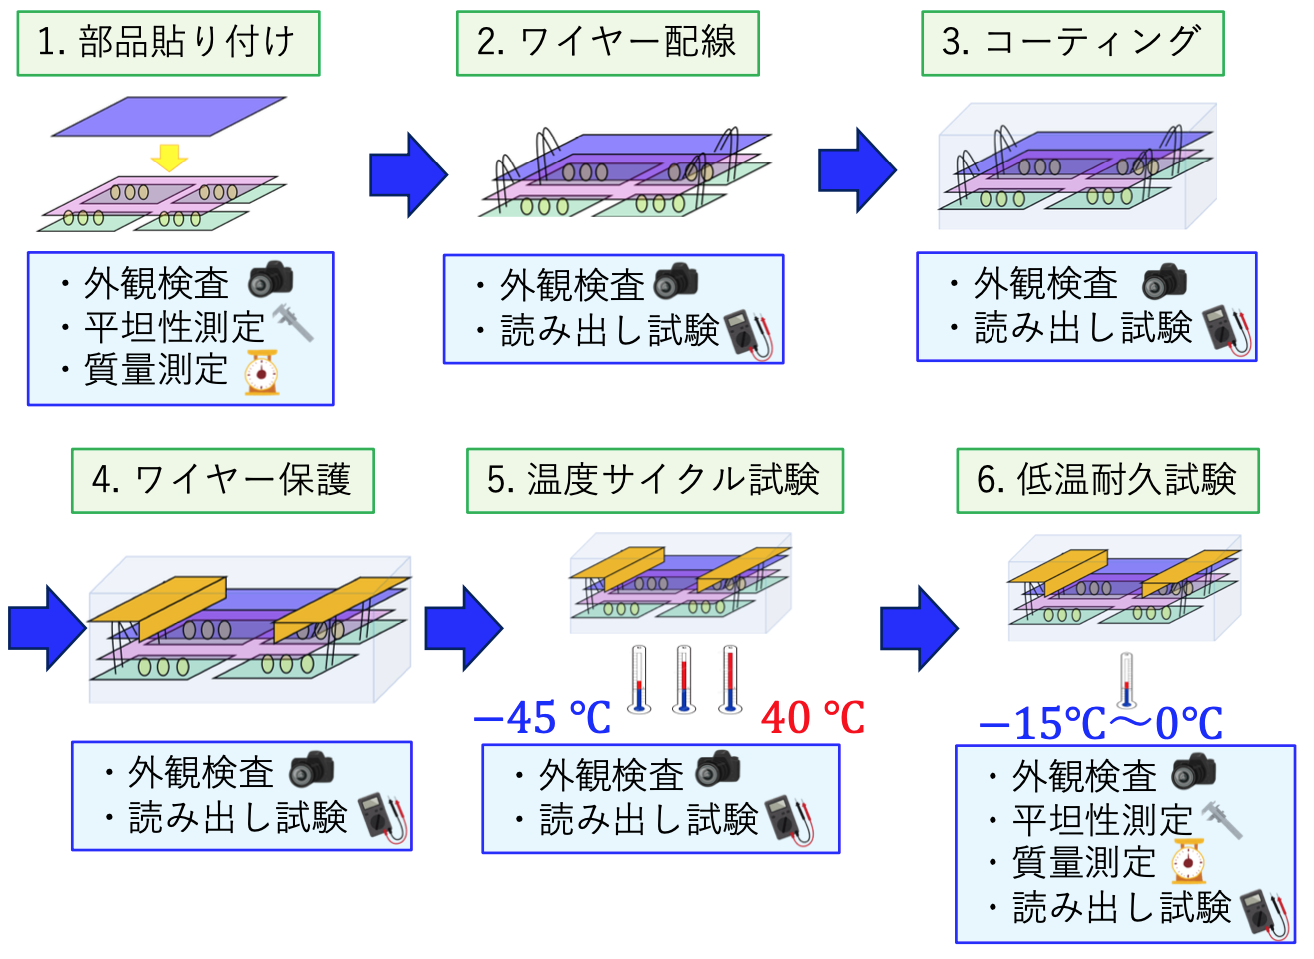
\includegraphics[height=2.3cm,keepaspectratio]{module_flow.png}
  \caption[ピクセル検出器の組み立て工程]{ピクセル検出器の組み立て工程。 }
  \label{fig:assemble}
\end{figure}


次世代ピクセル検出器の組み立て工程を\fref{fig:assemble}に示す。組み立て工程ではフレキシブル基板とベアモジュールの接着から始まり、ワイヤー配線、パリレン高分子によるコーティング、ワイヤー保護を行いピクセルモジュールが完成する。その後、温度サイクル試験および低温耐久試験において、運転時に想定される温度環境において組み立てたモジュールが運用できるかの試験を行う。本節では、組み立て工程、およびモジュールの温度耐久についての試験についての説明を示す。

\subsubsection*{ベアモジュール・フレキシブル基板の接合}

モジュールの組み立て工程は、組み立て機関に輸送されたベアモジュールとフレキシブル基板の接合から始まる。輸送された各部品の受け取り時の品質試験を行った後、ベアモジュールとフレキシブル基板の接合を行う。専用治具を用いて行うことにより、フレックス基板の位置の交差は$\pm 50\ \si{\micro m}$、平面度は$25\ \si{\micro m}$の精度で接合を行うことができる。

\subsubsection*{ワイヤーボンディング}

フレキシブル基板とASICを電気的に接合し、電源の供給や、ASICからの信号を読み出すため、フレキシブル基板とASIC間をワイヤーで接続する。この組み立て工程をワイヤーボンディングと呼ぶ。ワイヤーは直径$25\ \si{\micro m}$でのアルミ製であり、1モジュールに対して約$500$本用いられる。ワイヤーボンディング後からは、モジュールの電気的な読み出しが行うことができるため、これ以降の全ての組み立て工程では読み出し試験を行い正常に動作するかの確認を行う。

\subsubsection*{パリレンコーティング}

モジュールのセンサーとASICの端の部分での放電を防ぐこと、湿気や化学物質からの保護を目的としてパリレンコーティングを行う。パリレンはパラキシリレン系ポリマーの略である。パリレンは結晶性が高く絶縁耐力に優れ、周波数に依存せず低い誘電率・誘電正接特性を持っており、湿気や腐食性ガスへの耐性も併せ持つ。


\subsubsection*{ワイヤー保護}

ワイヤーは直径$25\ \si{\micro m}$と非常に細いため、力が加わると損傷してしまう可能性がある。特に、ITkを実装する際にモジュールのケーブルがワイヤーに触れてしまい、読み出しが正常にできなくなる恐れがある。このような問題を避けるため、\fref{fig:protection}に示すような構造体を用いて、ワイヤーを保護する。

\begin{figure}[tbp]
  \centering
  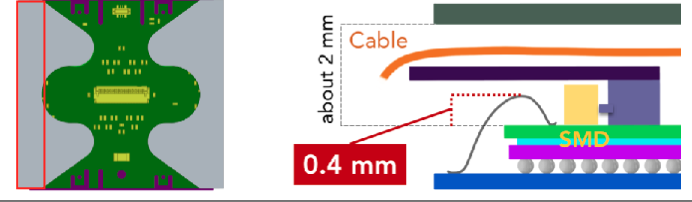
\includegraphics[height=4cm,keepaspectratio]{protection.png}
  \caption[ワイヤー保護用の構造体]{ワイヤー保護用の構造体。炭素系の素材であるCFRPを用いて作成する。図を作る。 }
  \label{fig:protection}
\end{figure}

\subsubsection*{温度サイクル}


組み立てたモジュールに対して、ITk実装後にされる特異的な温度変化のサイクルを行い、その後もモジュールが正常な応答をするか試験をする。温度変化の際、モジュールの部品間の熱膨張の違いにより熱応力が生じ、それが原因でバンプ接合部に剥がれが生じてしまうことがある。このようの温度サイクルによるモジュールの損傷がないことを確認する必要がある。

ITkの運転の切り替えが年間$10$回以上あるため、゙$10$年間の運転を想定すると$100$回以上の熱サイクルにさらされる。
そのため、量産における品質試験では、動作温度範囲$-45\ \si{\degreeCelsius}<T<40\ \si{\degreeCelsius}$の温度サイクルを$10$回、$-55\ \si{\degreeCelsius}<T<60\ \si{\degreeCelsius}$の温度サイクルを$1$回を行う。これらの温度サイクルの後にモジュールが正常に動作するかを確認するため、ASIC回路読み出し試験等を行う。モジュールの周囲温度を変える際には、恒温槽を用いて行う予定である。

\subsubsection*{低温耐久試験}

ITk運転におけるピクセル検出器の周囲温度は$-15\ \si{\degreeCelsius}<T<0\ \si{\degreeCelsius}$である。組み立てたモジュールが低温環境下において長時間正常に動作することを確認する試験が低温耐久試験である。
低温耐久試験では、温度制御筐体を用いてモジュールの周囲温度を$-15\ \si{\degreeCelsius}$に保ちつつASICの回路読み出し試験を行う。読み出し試験は1時間に1度行われる。
\begin{figure}[tbp]
  \centering
  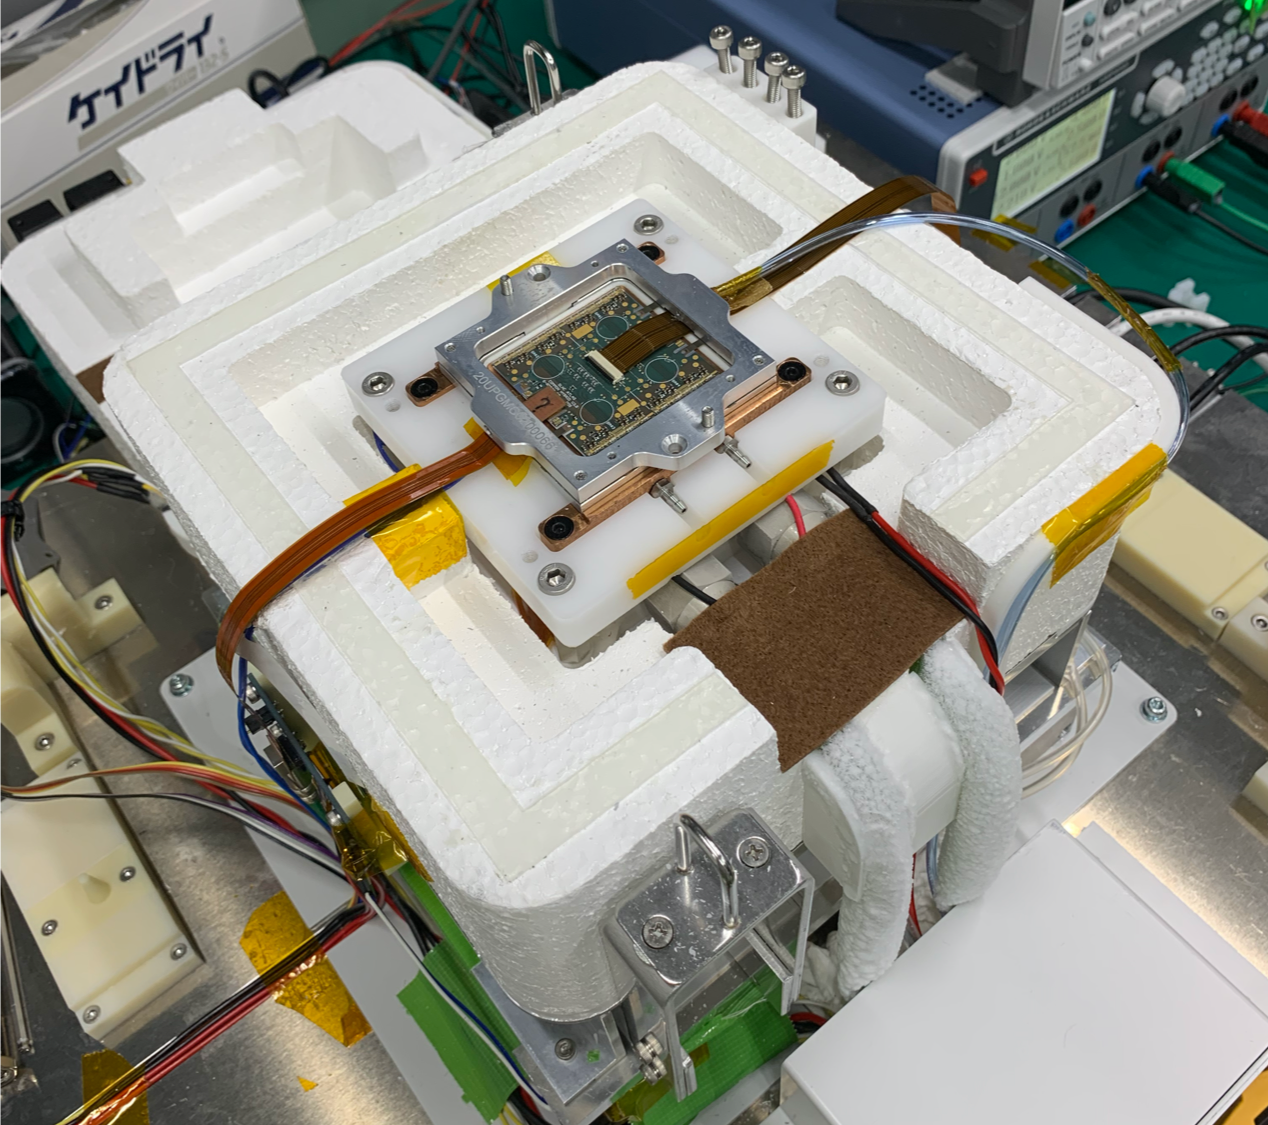
\includegraphics[height=7cm,keepaspectratio]{yomidashi.png}
  \caption[読み出し試験のセットアップ]{読み出し試験のセットアップ \cite{studyofID} }
  \label{fig:yomidashi}
\end{figure}
\begin{figure}[tbp]
  \centering
  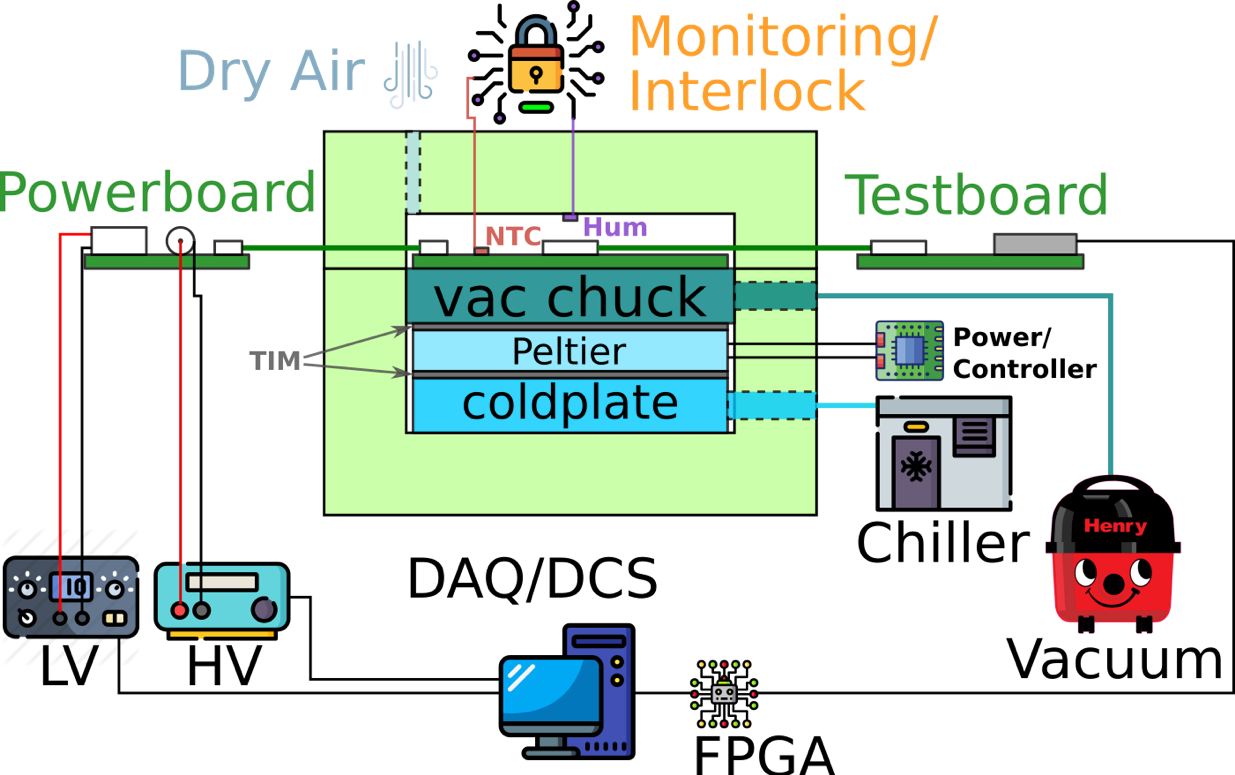
\includegraphics[height=7cm,keepaspectratio]{electrical_system.png}
  \caption[読み出し試験の全体図]{読み出し試験の全体図 \cite{studyofID} }
  \label{fig:electrical-system}
\end{figure}

長時間放置しつつ読み出し試験を行うため、インターロックシステム、機器の遠隔制御、温度制御筐体の遠隔監視等の技術が必要となる。
\\
\\
To do: ITk稼働の際にモジュール周囲温度が低い理由を二章に書く。\\
\url{https://arxiv.org/pdf/2003.00055.pdf}, \\
\url{https://iopscience.iop.org/article/10.1088/1748-0221/8/10/P10003/pdf}
\\




%------------------------------------------------------------------------------------------------------------------------
\section{品質試験}
\label{sec:QCtest}
%------------------------------------------------------------------------------------------------------------------------

モジュールの各組み立て工程の後に、モジュールが正常に動作するかを確認するために品質試験を行う。\fref{fig:assemble}に示したように、モジュールの外観検査は全ての工程で行われ、ASICの回路読み出し試験はワイヤー配線後の全ての工程で行われる。本節では、各品質試験項目の詳細を以下に示す。



%------------------------------------------------------------------------------------------------------------------------
\subsection{外観検査}
\label{sec:visualinsp}
%------------------------------------------------------------------------------------------------------------------------
モジュールの表面(フレックス基板側)をカメラを用いて撮影し、モジュールに損傷や汚れ等がないことを目視で確認する。特に、ASICとフレックス基板を電気的に接合するためのワイヤーの接着位置が正しいか、断線がないかを確認することが重要である。目視で確認する際は、モジュール全体の高解像度画像を36(縦横$6\times6$)分割して得られる拡大画像を用いて細かく検査を行う。また、ワイヤー部分については約$500$本のワイヤーを目視で漏れなく検査することは困難且つ労力を伴うため、ワイヤーの断線や接続部分のずれを自動で検知するアルゴリズムの開発が進んでいる。



%------------------------------------------------------------------------------------------------------------------------
\subsection{平坦性測定}
\label{sec:metrology}
%------------------------------------------------------------------------------------------------------------------------
モジュール上の3次元位置座標を取得することにより、歪み具合を計算することができる。\fref{fig:metrology}に平坦性測定結果を示す。

\begin{figure}[tbp]
  \centering
  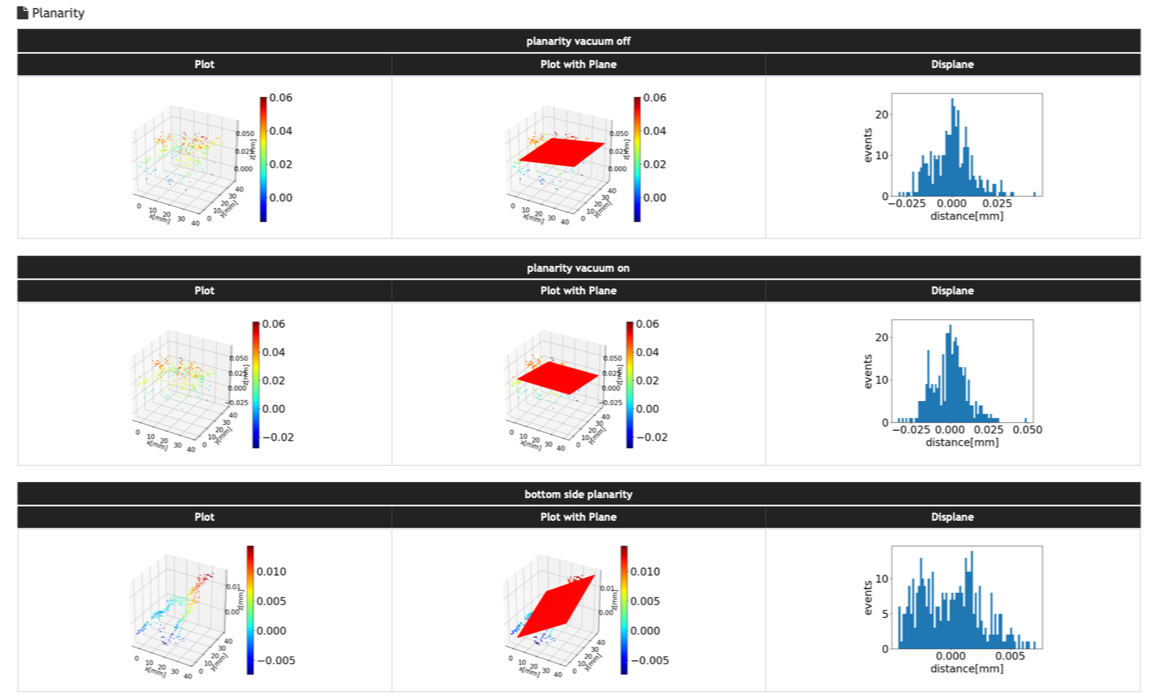
\includegraphics[height=7cm,keepaspectratio]{metrology.png}
  \caption[平坦性測定の結果]{平坦性測定の結果 }
  \label{fig:metrology}
\end{figure}


%------------------------------------------------------------------------------------------------------------------------
\subsection{質量測定}
\label{sec:mass}
%------------------------------------------------------------------------------------------------------------------------
質量測定では、モジュール全体の質量を測定する。各工程における質量の差を計算することにより、接着剤の質量やワイヤーの合計質量等を取得することができる。


%------------------------------------------------------------------------------------------------------------------------
\subsection{センサー IV特性}
\label{sec:sensoriv}
%------------------------------------------------------------------------------------------------------------------------
センサーの電流-電圧特性を調べることにより、モジュール製造工程におけるセンサーの損傷やHVのショートを確認することができる。
プラナーセンサーでは、leakage currentが$80\ \si{V}$で$2\ \si{\micro A}$、降伏電圧が$120\ \si{V}$、3Dセンサーについてはleakage currentが$25\ \si{V}$で$2\ \si{\micro A}$、降伏電圧が$35\ \si{V}$程度となるのが想定されうる結果である。また、測定はASICからの消費電力による発熱を避けるため、ASICへのLVを切った状態で行われる。
Todo: 2章を書きつつ、センサーの詳細を調べ直す。


%------------------------------------------------------------------------------------------------------------------------
\subsection{SLDO VI特性}
\label{sec:sldovi}
%------------------------------------------------------------------------------------------------------------------------
ITk実装時には、モジュールを直列に並べて電源の供給を行う。そのため、各モジュールに対する電源は定電圧ではなく、供給電圧はつなげるモジュールの数に依存してしまう。
ASIC回路内部で一定の電圧を供給するために、SLDO(\textbf{S}hunt \textbf{L}ow \textbf{D}rop \textbf{O}ut)という制御回路を用いる。SLDO制御回路が供給電流の一部を用いてデジタル回路、アナログ回路の動作電圧を生成し、余剰電流はグランドに捨てられる。ASICには二つのSLDO制御回路が搭載されている。1つはデジタル回路用、もう1つはアナログ回路用に用いる。\fref{fig:sldoref}にASICへの電流と、入力電圧$V_\mathrm{in}$、アナログ回路の出力電圧$V_\mathrm{analog}$およびデジタル回路の出力電圧$V_\mathrm{digital}$の例を示す。
\begin{figure}[tbp]
  \centering
  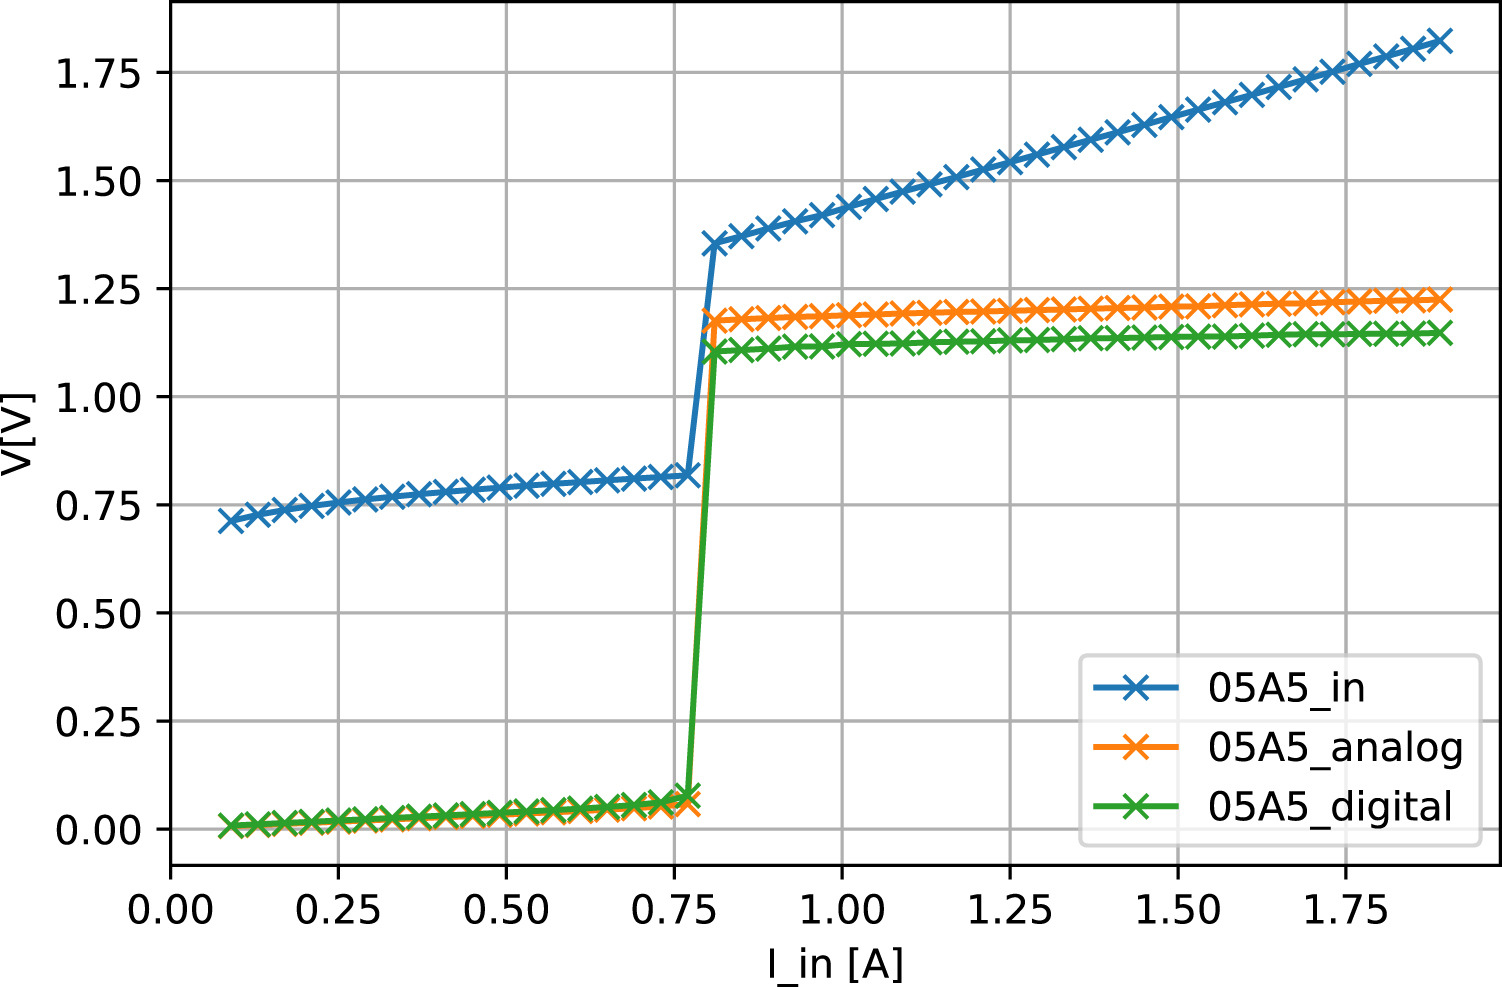
\includegraphics[height=7cm,keepaspectratio]{sldoref.jpg}
  \caption[SLDOVI]{SLDOVI}
  \label{fig:sldoref}
\end{figure}
この結果から、SLDO回路によりアナログ回路およびデジタル回路からの出力電圧は一定であり、制御回路が正常に動作していることがわかる。

さらに、SLDO VI特性についての品質試験を行う際には、ASICが低温においても正常に動作するかの試験も行う。モジュールの周囲温度を$-35\ \si{\degreeCelsius}$にし、デジタル回路の読み出し試験を行いモジュールが低温環境で動作することを確認する。正常に動作しない場合は$15\ \si{\degreeCelsius}$ずつ温度を上げて再び試験を行い、正常に動作を始める温度を記録する。
\begin{table}[htbp]
  \begin{center}
    \caption[Start at temperature]{Start at temperature criteria \cite{lingxin}}
    \label{tab:gradesldo}
    \begin{tabular}{|c|c|}
    \hline
      Temperature[$\si{\degreeCelsius}$] & Grade \\
    \bhline{1.5pt}
     $-35$ & $1$ \\
    \hline
     $-35 < T \leq -20$ & $2$ \\
    \hline
     $-20 < T \leq -5$ & $3$ \\
    \hline
     $-5 < T \leq 10$ & $4$ \\
    \hline
     $10 < T$ & $5$ \\
    \hline
    \end{tabular}
  \end{center}
\end{table}


%------------------------------------------------------------------------------------------------------------------------
\subsection{読み出し試験 \cite{electricaldoc}}
\label{sec:electricaltest}
%------------------------------------------------------------------------------------------------------------------------
モジュールに通電し、正常に読み出しができるか確認する。読み出し試験はITk運転時の温度環境を想定し、モジュールの周囲温度を変えつつ試験を行う。そのため、読み出し試験の際には低温耐久試験と同様に\fref{fig:yomidashi}の温度制御筐体を用いて試験を行う。設定温度は、低温におけるモジュール起動試験では$-35\ \si{\degreeCelsius}$ (正常に起動できない場合は$15\ \si{\degreeCelsius}$ずつ温度を上げて試験)、Threshold測定やToT測定等の通常の読み出し試験では$-20\ \si{\degreeCelsius}, 20\ \si{\degreeCelsius}$である。

読み出し試験に用いるDAQ(Data AcQuisition)として、YARR(\textbf{Y}et \textbf{A}nother \textbf{R}apid \textbf{R}eadout)を用いる。YARRとはASIC読み出しように開発されている。YARRを用いて行う、モジュールの読み出し試験の項目を以下に示す。

\begin{itemize}
  \item Digital scan \\
  Digital回路の応答を確認する。
  \item Analog scan \\
  Analog回路の応答を確認する。
  \item Treshold scan \\
  Thresholdを確認する。
  \item ToT scan \\
  ToTを確認する。
  \item Noise scan \\
  Noiseを確認する。
  \item Source scan \\
  放射線を照射し、応答を確認する。
\end{itemize}

また、これらのスキャン項目に加え、ピクセルのチューニングも行うことがある。
\begin{itemize}
  \item Global threshold tuning \\
  ASIC全体のピクセルにおけるThresholdを一括チューニングする。
  \item Pixel threshold tuning \\
  各ピクセル毎にThreshold値チューニングする。
  \item Global ToT tuning \\
  ASIC全体のピクセルにおけるToT値を一括チューニングする。
  \item Pixel ToT tuning \\
  各ピクセル毎にToT値をチューニングする。
\end{itemize}


\begin{table}[htbp]
  \begin{center}
    \caption[Powering overview for the on-detector system]{Powering overview for the on-detector system \cite{itk}}
    \label{tab:powering}
    \begin{tabular}{|l|l||l|}
    \hline
      \multirow{5}{*}{on-module} & Nominal LV current per module & $5.6\ \si{A}$ \\
    \cline{2-3}
      & LV nominal & $1.4\ \si{V}$ \\
    \cline{2-3}
      & Nominal Power per module & $7.85\ \si{W}$ \\
    \cline{2-3}
     & Chip power per area & $0.5\ \si{W/cm^2}$ \\
    \cline{2-3}
     & Sensor power per area & $< 0.1\ \si{W/cm^2}$ \\
    \hline
     \multicolumn{2}{|l||}{DCS power} & $0.15$-$0.28\ \si{W}$ per quad module \\
    \hline
     \multicolumn{2}{|l||}{Cooling system capability} & $0.7\ \si{W/cm^2}$ \\
    \hline
    \end{tabular}
  \end{center}
\end{table}


\begin{table}[htbp]
  \begin{center}
    \caption[Pixel Failure Categories]{Pixel Failure Categories}
    \label{tab:pixel-failure}
    \begin{tabular}{|l|l||l|}
    \hline
      Failure Name & Scan Type & Criteria \\
    \bhline{1.5pt}
      Digital Dead & Digital Scan & $\mathrm{Occupancy}<1\si{\%}$ of injections \\
    \hline
      Digital Bad & Digital Scan & $\mathrm{Occupancy}<98\si{\%}$ or $\mathrm{Occupancy}>102\si{\%}$ of injections \\
    \hline
      \multirow{2}{*}{Merged Bump} & Analog Scan & $\mathrm{Occupancy}<1\si{\%}$ of injections \\
       & Crosstalk Scan & $\mathrm{Occupancy}<80\si{\%}$ of $25\ \si{ke}$ injections \\
    \hline
      Analog Dead & Analog Scan & $\mathrm{Occupancy}<1\si{\%}$ of injections \\
    \hline
      Analog Bad & Analog Scan & $\mathrm{Occupancy}<98\si{\%}$ or $\mathrm{Occupancy}>102\si{\%}$ of injections \\
    \hline
      \multirow{2}{*}{Tuning Failed} & Threshold Scan & s-curve fit failed \\
       & ToT Test & ToT response is $0$ or $14\ \si{BCs}$ \\
    \hline
      Noisy & Noise Scan & $\mathrm{Occupancy}<10^{-6}$ hits per BC \\
    \hline
      Disconnected Bump & Source Scan & $\mathrm{Occupancy}<1\si{\%}$ of mean Occupancy \\
    \hline
      High Crosstalk & Crosstalk Scan & $\mathrm{Occupancy}>0$ with $25\ \si{ke}$ injection \\
    \hline
    \end{tabular}
  \end{center}
\end{table}

%------------------------------------------------------------------------------------------------------------------------
\subsection{モジュール特性}
\label{sec:module-prop}
%------------------------------------------------------------------------------------------------------------------------
モジュールの特性として、以下のようのものが定義されている。
\begin{itemize}
  \item FE chip version \\
  モジュールの部品となっているASICの種類を入力する。現在行っている試作器はRD53Aであり、ITkに向けたモジュール量産ではITkpix\_v2を用いる予定である。
  \item Thickness \\
  センサーの厚さの情報を入力する。この特性に入力する値としては"thin"と"thick"があり、それぞれセンサーの厚みが$150\ \si{\micro m}$と$300\ \si{\micro m}$である。
  \item Roof \\
  モジュールのワイヤー部を保護する構造体の有無を記録する。
  \item IrefTrim\\
  全てのDAC\footnote{D/Aコンバーターとも呼ぶ。}(\textbf{D}igital \textbf{A}nalog \textbf{C}onverter)は"IREF"と呼ばれるグローバルなレファレンスから$4\ \si{\micro A}$の電流を生成する。IrefTrimはワイアー接合の際に4bitの値で決められる。
  \item Pull-up registor\\
  Compare VREF\_A\_Trim at DAC count 16 with VDDA on hybrid after power-up \\
  For the chip to start up, VDDA > 1.14A\\
  If this is lower, you need to add a pull-up resistor!\\
  NTCに関係がある? \\
  \tref{tab:pull-up}
  \item PCB-Bare Orientation \\
  フレックス基板とベアモジュールの向きが正しいか確認する。
\end{itemize}

\subsubsection{Iref Trim}
\begin{figure}[tbp]
  \begin{minipage}[b]{0.45\linewidth}
    \centering
    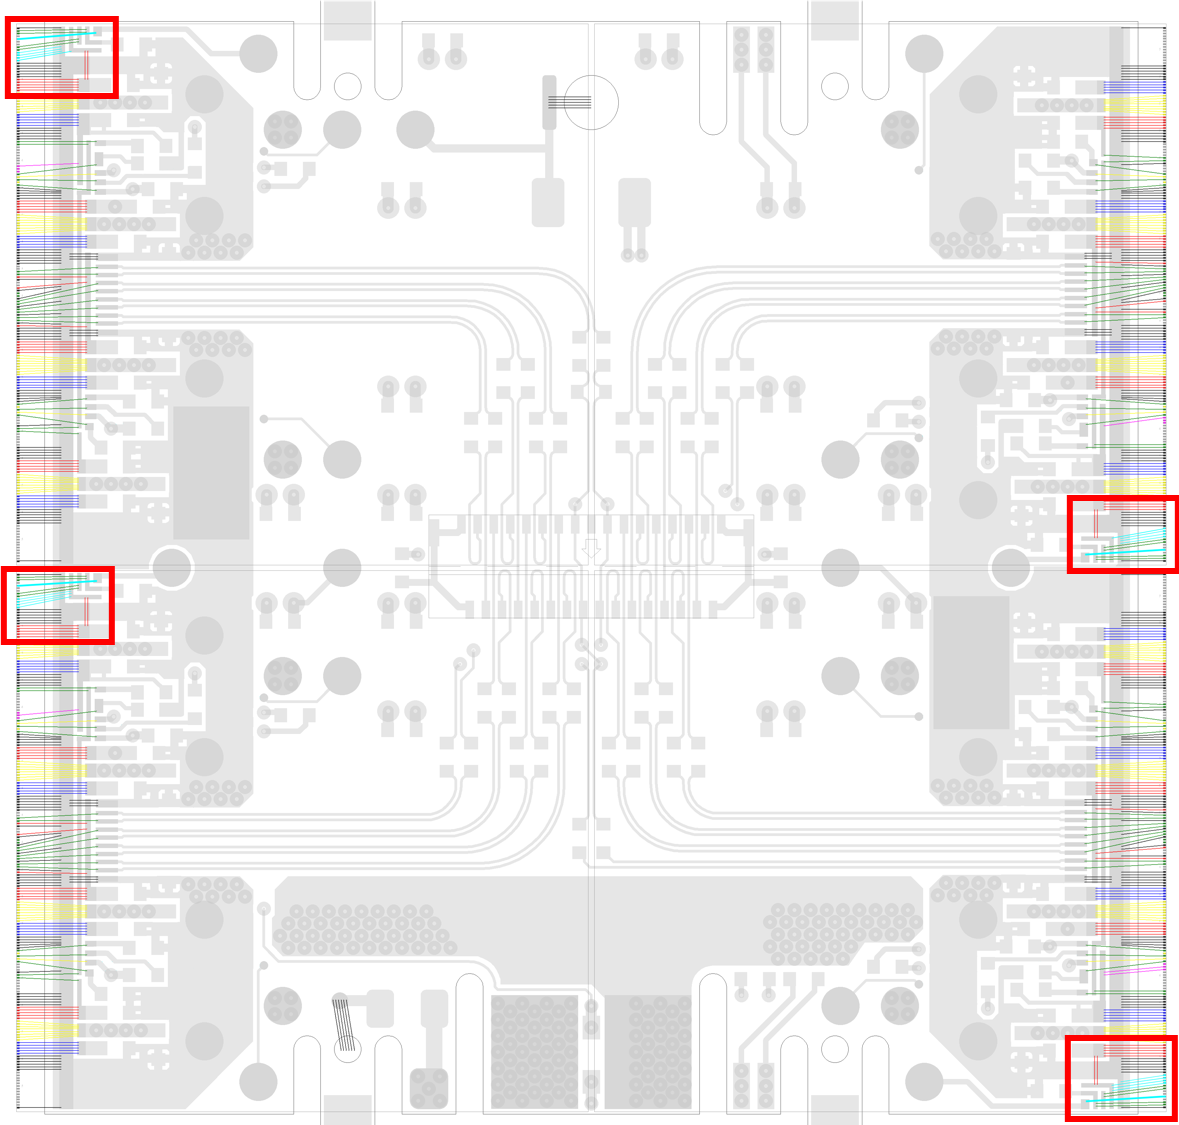
\includegraphics[keepaspectratio, scale=0.25]{iref_module.png}
  \end{minipage}
  \begin{minipage}[b]{0.45\linewidth}
    \centering
    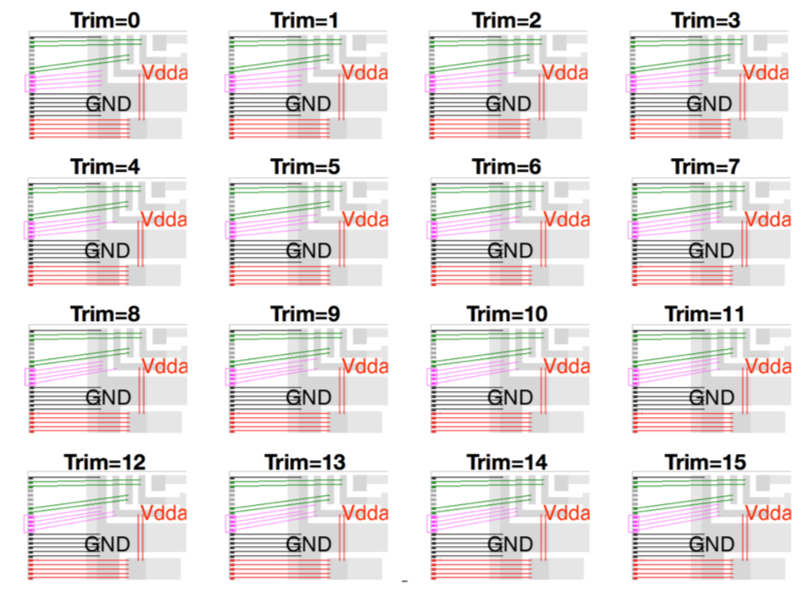
\includegraphics[keepaspectratio, scale=0.5]{iref_detail.png}
  \end{minipage}
  \caption{クアッドモジュールのIref Irim部分を表す部分(左図)とワイヤーの配線とIref値の関係。ピンク色のワイヤーの配置により4bitのIref値を表すことができる。}
  \label{fig:iref-detail}
\end{figure}

ワイヤーボンディング後に、Iref Trim値を確認する。


\subsubsection{Pull-up Register}
\begin{figure}[tbp]
  \centering
  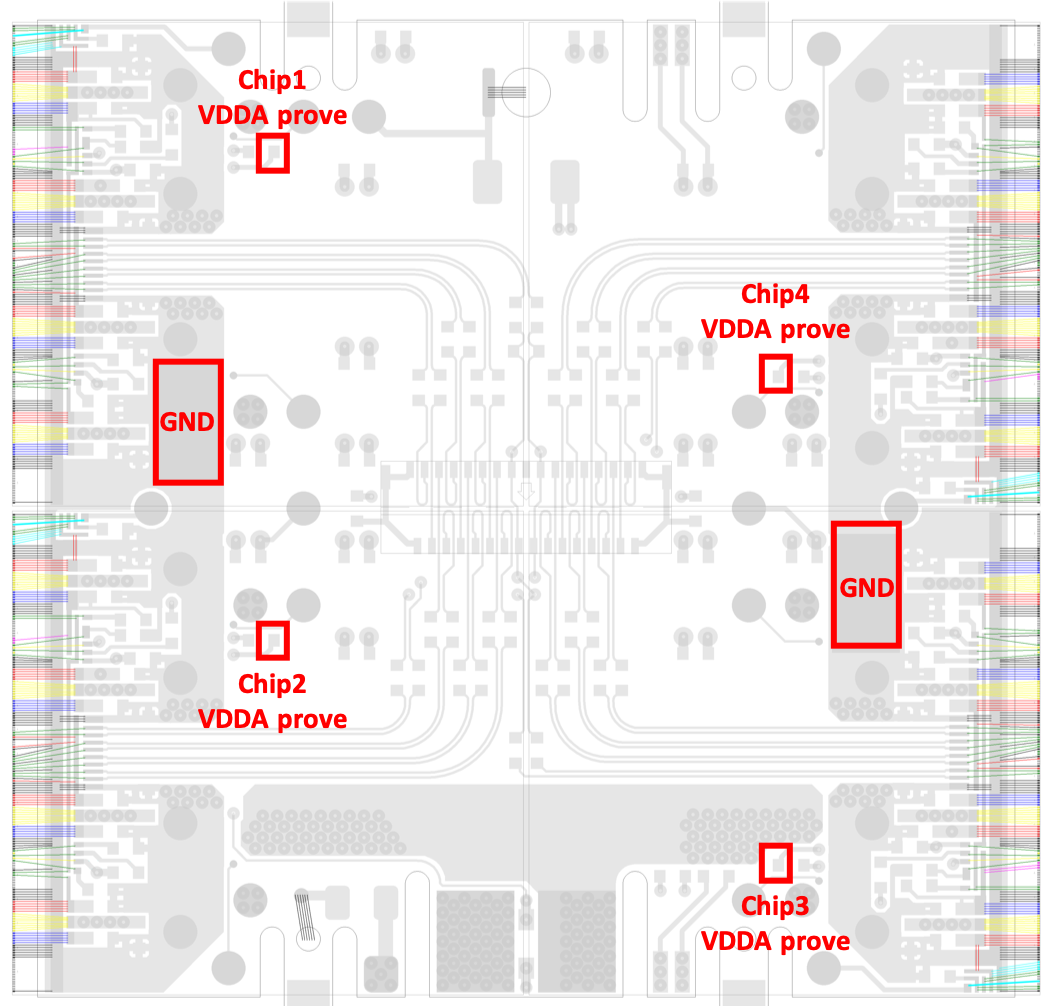
\includegraphics[height=6cm,keepaspectratio]{pullup.png}
  \caption[pull-up Resistor]{Pull-up Registor}
  \label{fig:pillup}
\end{figure}


\begin{table}[htbp]
  \begin{center}
    \caption[Pull-up Grade]{Pull-up Grade}
    \label{tab:pull-up}
    \begin{tabular}{|c|c|c|c|}
    \hline
      Start-up VDDA [\si{V}] & Pull-up Resistorが必要か & Pull-up Resistorの値 [$\si{\ohm}$] & VDDA no zouka\\
    \bhline{1.5pt}
     $V_\mathrm{DDA}\leq 1.09$ & Yes & 150 & 0.1 \\
    \hline
     $1.09 < V_\mathrm{DDA} \leq 1.14$ & Yes & 300 & 0.05 \\
    \hline
     $1.14 < V_\mathrm{DDA}$ & No & n/a & n/a \\
    \hline
    \end{tabular}
  \end{center}
\end{table}

\subsubsection{Bare PCB Orientation}
ベアモジュールの見た目は\fref{fig:bare}のように、$180\si{\degree}$回転対称になっている。そのため、フレックス基板とベアモジュールの貼り付け工程で誤って$180\si{\degree}$回転した状態で接合してしまうことがある。この誤りは、ワイヤー配線後に行う読み出し試験の際に初めて確認される。その場合は、ベアモジュールとフレックス基板の向きについての特性を書き直す必要がある。

%------------------------------------------------------------------------------------------------------------------------
\section{量産における試験結果管理}
\label{sec:production-manage}
%------------------------------------------------------------------------------------------------------------------------
各モジュールに対して、各組み立て工程および温度耐性についての品質試験を行い合計$30$個程度の試験を行う。試験項目によって結果データの形式は異なる。各品質試験のデータの形式およびデータサイズを\tref{tab:DBdata}に示す。
\begin{table}[htbp]
  \begin{center}
    \caption[品質試験のデータ]{品質試験のデータ}
    \label{tab:DBdata}
    \begin{tabular}{|l||l|c|c|}
    \hline
      試験項目 & 内容 & データ形式 & データサイズ\\
    \bhline{1.5pt}
     読み出し試験 & ASIC上の各ピクセルの結果 & JSON file & $629\ \si{MB}$ \\
    \hline
    \end{tabular}
  \end{center}
\end{table}
品質試験結果に加えて、ワイヤー配線をした後に確認できる、モジュール特性についてのデータも適切に管理する必要がある。

ITkのために世界各地の組み立て機関においてモジュールの量産およびそのための品質管理試験を行う。各組み立て機関では$\mathcal{O}(100)\sim \mathcal{O}(1000)$のモジュールの量産を行う予定であり、最も量産数が多いのは日本の高エネルギー加速器研究機構(KEK)における約$2000$個のモジュールの量産である。KEKにおける量産についてデータサイズは$??\ \si{TB}$になると想定される

ITkの製造に関係するモジュール情報や品質試験の結果は、チェコに設置されている中央のデータベースに保存する必要がある。そのため、各研究機関においてモジュール情報と品質試験結果を統一的に管理する必要がある。しかし、各モジュールにおいて$30$程度の試験項目がありデータの形式が異なること、さらに各研究機関で組み立てるモジュール数が多いことから、各研究機関独自のシステムを用いてデータ管理すると以下のような問題が想定される。
\begin{itemize}
  \item データの不整合 \\
  各研究機関において独自のシステムを用いると、試験結果の管理方法が異なることから他の機関との結果の比較が困難になる。モジュールを他研究機関に送った際に、輸送中にモジュールに損傷がないことを確認するために受け取り試験(レセプション試験)を行う。輸送前後の試験結果を比較を行うが、その際に試験結果の形式が異なると比較前に結果を整形する必要があり、試験機関の数だけ整形しなければならないため非常に面倒である。
  \item データの重複 \\
  試験結果やモジュール情報を共有した際、既にそのデータが存在すると使用しているPCのディレクトリ構造の違いにより別のデータと認識してしまいデータの重複が発生してしまう可能性がある。そのため、別の研究機関や異なるサーバーでデータを共有する際に、適切に管理する必要がある。
\end{itemize}

上記の問題を解決するために、各モジュール組み立て機関において適切にデータ管理を行うことを目的として、データベースシステムの開発を行っている。

このシステムについて、次章において説明する。

\newpage
